\documentclass[main.tex]{subfiles}
\begin{document}
\subsection{Con trỏ cơ bản}
Cho biết kết quả in ra màn hình của các đoạn code dưới đây:
\begin{enumerate}
    \item \begin{minted}{cpp}
float a = 15.75;
float* p = &a;
*p += 4;
cout << a;
\end{minted}
    \item \begin{minted}{cpp}
int a[] = {2, 5, 7, 1, 6};
int* p = a;
*(p + 1) += *a;
cout << *(a + 1);
\end{minted}
    \item \begin{minted}{cpp}
int a[] = {2, 5, 7, 1, 6};
int** p = &a;
(*p)[4] = *((*p) + 1);
cout << a[4] << endl;
\end{minted}
    \item \begin{minted}{cpp}
int a[][3] = { {4, 7, 2}, {5, 8, 1} };
cout << *(*(a + 1) + 2);
\end{minted}
\end{enumerate}
%%%%%%%%%%%%%%%%%%%%%%%%%%%%%%%%%%%%%%%%%%%%%
\subsection{Con trỏ nâng cao}
Hãy viết các đoạn code để cấp phát và giải phóng bộ nhớ và nhập nội dung cho các mảng động sau:
\begin{enumerate}[label=\alph*.]
    \item Mảng nguyên một chiều có $n$ phần tử. 
    \item Ma trận thực $M\times N$.
    \item Mảng có $n$ chuỗi kí tự, mỗi chuỗi có độ dài khác nhau nhập từ bàn phím.
\end{enumerate}
\textit{Lưu ý: Kích thước của các mảng trên được nhập từ bàn phím.
}
%%%%%%%%%%%%%%%%%%%%%%%%%%%%%%%%%%%%%%%%%%%%%
\subsection{Danh sách liên kết}
Một danh sách liên kết đơn có thành phần dữ liệu là số nguyên dương được mô tả như sau:
\begin{minted}{cpp}
struct List {
    Node *head;
}
struct Node {
    int data;
    Node *next;
}
\end{minted}
Hãy viết hàm \mintinline{cpp}{void makeOdd(List &list);} xử lý các số chẵn trong danh sách bằng cách phân tách số chẵn thành tổng 2 số lẻ có giá trị cách nhau không quá 2 đơn vị (thứ tự từ bé đến lớn)(Không dùng lại node số chẵn, mà tạo lại 2 node mới cho số lẻ), đồng thời sau đó loại bỏ các Node có dữ liệu giống nhau nằm liền nhau.
\begin{minted}{text}
Input:  3   8   6   1
Output: 3   5   3   1
\end{minted}

\begin{figure}[H]
\centering
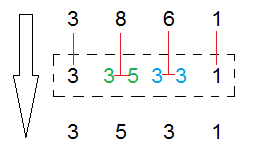
\includegraphics[width=0.4\textwidth]{image/q_DSLK.png}
\end{figure}
%%%%%%%%%%%%%%%%%%%%%%%%%%%%%%%%%%%%%%%%%%%%%
\subsection{Ngăn xếp, hàng đợi}
\subsubsection{Ngăn xếp}
\textit{Bài toán bên dưới nằm trong Interview Preparation Kit của \code{hackerrank}, nên các bạn có thể hình dung khi phỏng vấn xin việc thì những bài toán họ cho các bạn cũng nằm ở mức độ tương tự như thế này. Link: \href{https://www.hackerrank.com/challenges/balanced-brackets/}{Balanced Brackets}}.

Cho một chuỗi chứa các cặp dấu ngoặc \code{() [] \{\}}. Một chuỗi các dấu ngoặc được gọi là ``hợp lệ'' nếu như với mỗi dấu mở ngoặc thì nó sẽ có một dấu đóng ngoặc cùng loại tương ứng.

Ví dụ: các chuỗi sau là hợp lệ: \code{()[]\{\}, \{[()]\}, ([]\{\}), [\{()\{\}\}], ...}. 

Hãy thực hiện các yêu cầu sau:
\begin{enumerate}[label=\alph*.]
    \item Trình bày ý tưởng để biết được một chuỗi các cặp dấu ngoặc có là hợp lệ hay không?
    \item Viết hàm \mintinline{c}{bool checkBracketPairs(string str);} kiểm tra tính hợp lệ của một chuỗi như mô tả ở trên.
\end{enumerate}
\textit{Gợi ý: dấu mở ngoặc nào xuất hiện trước sẽ luôn được đóng trước.}

%%%%%%%%%%%%%%%%%%%%%%%%%%%%%%%%%%%%%%%%%%%%%
\subsection{Đệ quy và giải thuật sắp xếp}
\textit{Đề thi cuối kỳ KTLT lớp 19CTT4 (2020).}

Cho cấu trúc danh sách liên kết như sau:
\begin{minted}{cpp}
struct List {
    Node *head;
}
struct Node {
    int data;
    Node *next;
}
\end{minted}
Hãy viết \textbf{hàm đệ quy} Selection Sort để sắp xếp danh sách liên kết trên tăng dần?
%%%%%%%%%%%%%%%%%%%%%%%%%%%%%%%%%%%%%%%%%%%%%
\subsection{Quy hoạch động}
Cho một giỏ có vô hạn đồng xu gồm nhiều mệnh giá khác nhau, các loại mệnh giá được lưu trong một mảng \code{int a[]} có kích thước \code{m} (mảng được sắp xếp tăng dần). Cho một món hàng có giá tiền là \code{n} (xu), hãy tìm ra cách lấy các đồng xu từ giỏ trên (với mỗi mệnh giá có thể lấy một hoặc nhiều đồng xu) để trả tiền cho món hàng đó sao cho \textit{số lượng đồng xu là nhỏ nhất}?

Ví dụ:
\begin{figure*}
\centering
\begin{tabular}{|l|l|l|}
\hline
a           & n & Output\\
\hline
\{2, 3, 4\} & 1 & \code{Khong duoc} \\
\{2, 3, 4\} & 5 & 2 3    \\
\{2, 3, 4\} & 7 & 3 4  \\
\{2, 3, 4\} & 4 & 4  \\
\{2, 3, 4\} & 9 & 2 3 4 \\
\{2, 3, 4\} & 15 & 4 4 4 3 \\
\{2, 3, 5\} & 15 & 5 5 5 \\
\hline
\end{tabular}
\end{figure*}

\newpage
\subsection{Bài tập tự luyện ở nhà}
\subsubsection{Cấp phát động}
Cho cấu trúc số phức như ở bên dưới, hãy viết \textbf{hàm} cấp phát bộ nhớ động và giải phóng bộ nhớ cho một ma trận phức có kích thước $M\times N$ nhập từ bàn phím. Hãy viết thêm các \textbf{hàm} nhập, xuất dữ liệu và tính tổng các phần tử cho ma trận này. 
\begin{minted}{c}
struct ComplexNumber {
    float Re;
    float Im;
};
\end{minted}


\subsubsection{Ngăn xếp}
\textit{Bài toán bên dưới nằm trong Interview Preparation Kit của \code{hackerrank}, nên các bạn có thể hình dung khi phỏng vấn xin việc thì những bài toán họ cho các bạn cũng nằm ở mức độ tương tự như thế này. Link: \href{https://www.hackerrank.com/challenges/ctci-queue-using-two-stacks}{Queues: A Tale of Two Stacks}}.

\textbf{Sử dụng 2 stack, hãy ``giả lập'' ra một hàng đợi} và thực hiện các yêu cầu sau:
\begin{enumerate}[label=\alph*.]
    \item Nêu ý tưởng thực hiện.
    \item Tạo ra struct \code{QueueFS} (queue from stacks) chứa 2 stack kiểu nguyên và viết 3 hàm \code{enqueue}, \code{dequeue} và  \code{peek} để thao tác với queue vừa tạo ra đó.
    \item (Đọc thêm) Hãy xác định điểm chưa tối ưu của giải pháp vừa thực hiện và tối ưu nó.
\end{enumerate}
\textit{Gợi ý: Khi ta sử dụng stack để ``giả lập'' một queue, vì 2 kiểu dữ liệu này ngược nhau nên khi enqueue vào queue thì phần tử đó sẽ nằm trên đỉnh stack. Tuy nhiên, lúc ta muốn dequeue thì phần tử cần dequeue lại nằm dưới đáy stack. Do đó ta cần 2 stack để giải quyết bài toán này.}

\subsubsection{Đệ quy}
Game Minesweeper có một thuật toán rất hay đó là thuật toán vết dầu loang. Thuật toán được mô tả như sau:
Có hai ma trận 2 chiều, một ma trận \code{int} được lưu trữ các số và boom \code{(-1)}, một ma trận \code{bool} để lưu trữ thuộc tính ô có được mở hay không.
Khi ô được chọn là boom thì sẽ trả ra kết quả \code{BOOM!!}.   
Khi ô được chọn không phải boom thì nó sẽ loang ra:  
\begin{itemize}
    \item Nếu ô có boom thì nó sẽ không được mở.
    \item Nếu ô không có boom và không có số thì thuật   toán loang sẽ tiếp tục cho ô đó.
    \item Nếu ô không có boom và có số thì chỉ mở ô đó.
\end{itemize}
Hãy viết thuật toán đệ quy cho hàm mở ô sử dụng thuật toán loang.

\subsubsection{Quy hoạch động}
Cho một số nguyên dương $m$ ($m>100$), có thể biểu diễn $m$ thành tổng 3 số nguyên tố hay không? Nếu được hãy in 3 số nguyên tố đó ra. 

\end{document}